\chapter{Quelles traces les interactions biotiques laissent-elles dans les données de co-occurrence des espèces?}
\label{chap3}

\section{Résumé en français du troisième article}

Dans ce troisième article, je me suis me intéressé aux données de co-occurrence.
Ces données, très importantes en biogéographie, sont des enregistrements
de présences et d'absences pour un certain nombre d'espèces
le long d'un gradient géographique (par exemple latitudinal).
On dispose alors d’un grand nombre de sites sur lesquels les conditions abiotiques
varient et pour lesquels nous disposons également de la connaissance
d’une partie du contexte biotiques (les présences de différentes espèces).
En plus de ces informations, les jeux de données présentés sont munis
d’observations relatives aux information réelles avec lesquelles il es possible
de construire des réseaux d'interaction. J'ai donc analysé la co-occurrence à la
lumière des propriétés des réseaux de type trophiques, mutualistes ou de compétition
avec des espèces plus ou moins généralistes ce qui m’a permis de tester les
hypothèses faîtes au chapitre \ref{chap2}.


Nos résultats montrent que les interactions ont un effet sur la co-occurrence
mais que la détection de cet effet est délicate quand 1) les espèces sont éloignées
dans le réseaux :les interaction indirectes sont finalement presque
indétectables et 2) quand les interactions sont nombreuses, il est plus
difficile de trouver des signaux de co-occurrence \footnote{Il s'agit de
dévations par rapport à des attendus sous l'hypothèse que n'ont pas d'influence}
pour les espèces généralistes. De plus, en intégrant la similarité des facteurs
abiotiques pour les différents sites, je montre que les signaux de
co-occurrence s’affaiblissent et parfois disparaissent. Mes résultats suggèrent
donc qu’en utilisant des facteurs abiotiques pour inférer les probabilités de
co-occurrence, une partie du lien entre les espèces est capturée, mais cette
part est entachée d’une grande incertitude. Ceci vient questionner la
qualité des prédictions données par les modèles classiques de distribution
d'espèces actuellement utilisés. Nos résultats jettent une lumière forte
intéressante sur un débat classique en
écologie concernant la détection des interaction à partir des aires de
distribution. Nous montrons que la configuration du réseau est aussi
importante et qu’il ne faut pas trop rapidement conclure que les espèces sont
indépendantes, ce qui est souvent à la base des projections que nous faisons
pour anticiper les changements de biodiversité.



\subsection{Publication envisagée}

Le travail ici présenté a été rendu possible grâce à une collaboration entre différents
chercheurs menée avec Dominique Gravel. Les jeux de données que j'ai analysé
sont, en effet, difficiles à trouver et particulièrement riche en informations.
Je remercie tous les chercheurs qui m'ont accordé leur confiance
pour analyser les données et toutes les personnes qui ont contribué à la collecte
des données. Pour les données sur les colibris et les plantes des Caraïbes,
je remecie Bo Dalsgaard, Louise J. Lehmann, Ana M. Martín González,
Andrea Baquero, Allan Timmermann. Pour les données sur les communautés des feuilles de Saules,
je remercie Tomas Roslin. Pour les données sur les communautés microbiennes des
Sarracénies (\emph{Sarracenia purpurea}), je remercie Benjamin Baiser.
Pour les données du Suivi Temporel des Oiseaux Communs (STOC), je remercie Wilfried Thuiller
et pour les données des arbres, je remercie Dominique Gravel et Steve Vissault.

L'article qui suit est le fruit de discussions avec Dominique Gravel sur le type
d'analyse à mener pour donner suite au chapitre \ref{chap2}. Je me suis occupé
de l'ensemble des analyses, des figures, de la rédaction de la première version
relue par Dominique Gravel. J'ai également bénéficié d'une précieuse et
attentive relecture de David Beauchesne que je merci chaleureusement.
Due à la qualité des jeux de données, à l'originalité de nos analyses et
nos résultats, je nourris l'espoir que mes résulats intéresseront
une revue généraliste. C'est pour cela que le chapitre est dans un format court avec une
longue section "Supplementary information" (SI, \ref{chap3si}). Se confronter
à la rédaction en format court fut aussi un exercie très enrichissant bien que délicat.




\subsection{Traduction du résumé en anglais}

Un problème majeur en biogéographie et en modélisation de la biodiversité
est de savoir si la co-occurrence des espèces contient une trace des
interactions. L'hypothèse conventionnelle affirme que les interactions
négatives et positives conduiraient respectivement à des répulsions et
des attractions. La rareté des jeux de données combinant des distributions
à larges échelles avec des données d'interactions a longtemps empêché
les biogéographes d'obtenir des idées claires sur ce problème. Pour répondre
à cette question, nous avons utilisé cinq jeux de données sur un large
gradient de conditions climatiques incluant des informations sur les interactions écologiques,
représentant un total de 793 espèces pour 354015 observations de co-occurrence.
Nous avons comparé la co-occurrence des pairs d'espèces interagissant avec
celle de paire d'espèces n'interagissant pas en intégrant ou non les
variables abiotiques. Nous avons trouvé un effet des interactions sur la
distribution des espèce de co-occurrence brute mais pas de preuve d'un tel
effet lorsque les variables abiotiques étaient intégrées. De plus, nous avons
trouvé que certaines propriétés du réseau d'interactions pouvaient masquer l'impact
des interactions sur la co-occurrence. Nous avons ainsi montré que plus le nombre
d'interactions qu'une espèce entretenait était grand, plus notre capacité
à détecter le signal dans les données d'interactions statiques était faible.
De plus, nous démontrons clairement que le signal de co-occurrence entre un
prédateur et ses proies disparait quand la proportion de sites couverts par
l'ensemble de proie augmente. Dans un contexte où les écosystèmes sont
fortement perturbés par l'activité humaine, nos résultats insistent
sur le besoin d'intégrer les processus écologiques dans les
modes de distribution d'espèces pour mieux prédire la biodiversité de demain.






\emph{Les sections qui suivent sont celles de l'article envisagé.}


\newpage
\section{Title}\label{title}

Do interacting species co-occur differently from not-interacting
species?

\section{Abstract}\label{abstract}

A major problem in biogeography and biodiversity modeling is whether
species co-occurrence holds an imprint of ecological interactions. The
conventional hypothesis poses that negative and positive interactions
should yield repulsion and attraction, respectively. The scarcity of
datasets combining broad scale distributions with observed interactions
has long prevented biogeographers from obtaining clear insights into
this problem. To address this question, we compile five datasets of
species distribution over a large range of climatic conditions, along
with their ecological interactions, representing of a total 793 species
and 354015 occurrence observations. We compared co-occurrence of
interacting versus non-interacting pairs of species accounting or not
for abiotic variables. We found an effect of interactions on species
distribution in raw co-occurrence data but no clear evidence of such
effect once when accounted for abiotic factors. Moreover we found that
some properties of the network of interactions could hide the impact of
interactions on co-occurrence. We showed that the larger the number of
interactions a species is experiencing, the weaker our ability to detect
signals in static co-occurrence data. Also, we clearly demonstrate that
the signal of co-occurrence between a predator and its preys vanishes
when the proportion of the sites covered by the set of preys increases.
In a context where ecosystems are dramatically disturbed by human
activities, our results emphasize the need for integrating ecological
processes into distribution models to better predict tomorrow's
biodiversity.

\section{Introduction}\label{introduction}

Biogeographers are still debating about whether biotic interactions at
the local scale impact large scale species distribution. If this is
indeed the case, then we should expect pairs of species to exhibit
non-random distribution at the large spatial scale. The observation of
independent species occurrences would therefore support the use of
classical species distribution models \citep[hereinafter
SDMs,][]{Elith2006} and confirm scenarios that have been proposed over
the last decade \citep{Thuiller2005, Thuiller2011, Albouy2012}. On the
other hand, the observation of occurrence clearly related to
interactions would give credit to methods interpreting co-occurrence as
a proxy for ecological interactions \citep{Morales-Castilla2015} and
encourage the use of joint species distribution models \citep[hereafter
JSDM,][]{Ovaskainen2010, Pollock2014}. In order to test whether
interactions influence species distributions, the simplest avenue is to
investigate species co-distribution in light of their ecological
relationships. Such investigations started with Diamond's original study
stating that species interacting by competition should avoid each other
in space, leading to a `checkerboard' distribution \citep{Diamond1975}.
This idea was rapidly criticized for the lack of an adequate null
hypothesis \citep{Connor1979, Gilpin1982} and has led to a major
controversy that has lasted more than 30 years \citep{Connor2013} and
has underlined the need for null models in ecology
\citep{Connor1983, Gotelli2000}. Furthermore, the absence of adequate
datasets has long prevented this hypothesis to be test appropriately.

Species ranges are very often inferred from the realized distribution,
which results from the joint impacts of abiotic and biotic environmental
factors along with dispersal limitations and historical contingencies
\citep{Pulliam2000, Holt2009, Godsoe2010a, Araujo2014}. Finding evidence
of the effect of species interactions on distribution may prove
technically difficult as it needs to discriminate the fundamental niche
from co-occurrence data (Box \ref{chap3box1}), which could explain the
scarcity of studies reporting such effect \citep[but
see][]{Gotelli2010}. Fortunately, recent developments in co-occurrence
theory promises novel avenues in which highly dimensional species
distribution data could be analyzed, accounting for the structure of the
network of ecological interactions \citep{Cazelles2016}. It has notably
been proposed that the higher the degree of a species, \emph{i.e} the
number of species with which it interacts, the weaker will be the
detection of a co-occurrence signal. The geographical range of a species
is indeed partially correlated with all the ranges of species it is
linked to, which should blur the signal the interactions leave on
pairwise co-occurrence. However, a signal may persist if the
co-occurrence of the focal species with the joint distribution of the
species it interacts with is considered.\\
Also, two co-occurring species may be part of the same ecological
network but separated by several interactions. For such case, it has
been suggested that the longer the shortest-path, \emph{i.e} the number
of links between two species, the smaller the signal of co-occurrence.
Hence, based on co-occurrence data and information pertaining to
ecological network, the hypotheses recently formulated on the signal of
co-occurrence can be tested (Box \ref{chap3box1}).

Despite the fantastic number of studies investigating co-occurrence in
order to understand community assembly, the hypothesis that species
interactions should result in non-random associations in space has never
been tested formally. It is rather implicitly assumed in every
investigation. Our objective in this study is therefore to test this at
the scale of species range. We analyzed species association within five
different datasets ranging from plant-seed dispersers, host-parasitoids,
microbes, birds and forest trees. We quantify co-occurrence and
conditional co-occurrence accounting for abiotic constraints for species
that are known to interact and known to not interact directly. This is a
unique opportunity to test the hypotheses recently developed. We report
some signal of positive co-occurrence among the datasets, suggesting a
difference between pairs of interacting and pairs of not-interacting
species. We also point out that the degree of a species in a network
influences our ability to detect significant associations. Moreover, we
discover a clear relationship between the strength of species
associations and the cumulated occupancy of the entire set of species
with which a species interact. However, all the signal we detected are
weakened or even disappear once abiotic similarities among site are
integrated. We further discuss the integration of biotic interactions in
distribution models in light of our results.

\section{Material and Methods}\label{material-and-methods}

\subsection{Datasets}\label{datasets}

We analyzed five datasets spawning a large diversity of organisms and
types of interactions (see Table \ref{tbl:datasets}), across an
extensive gradient of environmental conditions (see Fig. \ref{fig:maps}
and SI \ref{chap3si}). Our criteria for selecting datasets were as
follow: i) the occurrence data must have been collected at the local
scale, it could not be derived from range maps; ii) data included
observed absences; iii) occurrence was observed for all species:
interactions were known a priori; v) since we are computing
co-occurrences, which is typically a fairly rare event, we needed an
elevated number of sampling units. Direct interactions were documented
for four datasets and represented by networks of ecological
interactions: the Willow Leaf Network (WLN), the Pitcher Plants Network
(PPN), the Caribbean Hummingbirds Network (CHN), the French Breeding
Birds Survey (FBBS). We derived metawebs for each network, \emph{i.e},
the matrix recording all interactions, and computed three metrics among
species from a regional pool: the connectance of metawebs (proportion of
realized interactions), the degree of species (number of links for one
species) and the shortest-path between all pairs of species (the minimum
number of link from one species to the other, see SI \ref{chap3si}). For
the North American Trees (NAT) dataset, we approximated competitive
interactions by computing functional distance between every pair of
species (see Table \ref{tbl:rpkges} and Fig. \ref{fig:dendro}). A
similar proxy for ecological interactions was also computed for the FBBS
see SI \ref{chap3si}). Only species that were present at least on 1\% of
the total number of observations were considered for the analysis (see
SI \ref{chap3si}).

\subsection{Quantifying co-occurrence}\label{quantifying-co-occurrence}

For each pair of species \(i\) and \(j\), we computed the number of
observed co-occurrence \(O_{i,j}\) and the expected number of
co-occurrence under independent distribution \(E_{i,j}\) and the
standard deviation associated \(SD_{i,j}\). We report the Z-score
\(frac{O_{i,j}-E_{i,j}}{SD_{i,j}}\) \citep{Gilpin1982}, a standardized
metric of co-occurrence, with positive (negative) values indicating more
(less) co-occurrence relative to the random expectation. Expectations
were derived using three different methods. First, we assumed that all
sites were equivalent, meaning we ignored the potential influence of
abiotic conditions across the entire range. The observed co-occurrence
is an estimate computed from a limited number of observations
\citep{Gilpin1982, Veech2013} and therefore, we also considered an
hypergeometric distribution, which corrects for limited sample size (see
SI \ref{chap3si} for further details). We used two different SDMs in
order to account for the abiotic environment and correct the random
expectations, namely, Generalized Linear Model (hereafter GLM) and
Random Forest (hereafter RF - see SI \ref{chap3si} for more details and
Fig. \ref{fig:auc} for the assessment of models' performances). The
correction using SDMs accounts for the fact that species may co-occur
simply because they have similar abiotic requirements, irrespective of
if they interact or not.

\section{Results}\label{results}

Without accounting the abiotic context, we observe a difference in the
strength of spatial associations between interacting and not-interacting
species (Fig. \ref{fig:synth} panels A to D, white boxplots) for two out
of four datasets for which direct interactions were known. In all cases,
spatial associations were positive, indicating that interacting species
are co-occurring more often that randomly expected, irrespective of the
type of interaction. For the WLN, distinguishing herbivore-willow
interactions from herbivore-parasitoids revealed that the strength of
co-occurrence was greater for the former than the latter (Fig.
\ref{fig:shtpth} A-B). Interestingly, we noticed that detection of a
signal of interactions in co-occurrence became more difficult as the
mean degree of species in the dataset increased (Fig. \ref{fig:shtpth}
A-D). Therefore, based on co-occurrence data only, we conclude that
interactions affect co-occurrence, but that detection trend becomes
trickier in highly connected network.

We observed that the strength of spatial association was higher for
pairs of similar species (Fig. \ref{fig:synth} panels E and F) for the
NAT and FBBS datasets, for which we inferred a distance based on
functional traits. Functional similarity is often interpreted as a proxy
for competition strength \citep{Morales-Castilla2015}, which according
to Diamond's hypothesis, should provide a negative association.
Interestingly, we observe the opposite trend. This suggests that local
competition is poorly detectable at large scale, which is theoretically
supported \citep{Araujo2014}, and the positive associations are likely
the results of similar physiological requirements that cannot be taken
into account given the sets of abiotic variables we used. This is
further supported by the regressions of the Z-score against the distance
(see Fig. \ref{fig:distrev} A-D). We also note that results for the FBBS
dataset were identical irrespective the type of traits examined (Fig.
\ref{fig:dist}). Hence, the detection of interactions from co-occurrence
data varies according to the nature of the ecological relationships.

When we account for suitability discrepancies among sites using SDMs,
the co-occurrence signals we previously observed are weakened or
disappear. Co-occurrence distributions are shifted toward 0 and
dramatically shrunk (Fig. \ref{fig:synth} panels A to D, grey and dark
grey boxplots). The tendencies are stronger for the RF approach than for
the GLM one. The same trends are observed when we used functional
distance rather that interactions (Fig. \ref{fig:synth} panels E-F).

We investigated if the strength of associations between species
interacting indirectly decreases with the shortest path (Fig.
\ref{fig:shtpth}). We examined the co-occurrence distribution against
the shortest-path for pairs of: herbivores and willows in WLN (A),
herbivores and parasitoids in WLN (B), hummingbirds and hosts plants (C)
and all pairs in PPN (D). Without accounting for the climatic factors,
we observe a decrease of the standardized co-occurrence with an
increased shortest-path for three out of four occurrence datasets (Fig.
\ref{fig:shtpth} A-D, white boxplots). This was predicted by the theory,
but the observed decay is steeper than anticipated \citep{Cazelles2016}.
We observed a similar but weaker decay when all pairs of species were
taken into account (see Fig. \ref{fig:sht_pth2}). Moreover, when we
calculated the mean degree of predators (pollinators), we also found the
signal of co-occurrence stronger for specialists (Fig. \ref{fig:shtpth}
A) than for generalists (Fig. \ref{fig:shtpth} C), suggesting that the
abundance of interactions may prevent us from detecting them in static
occurrence data. Again, the tendencies observed are strongly weakened
when occurrence probability are derived from SDMs (Fig. \ref{fig:shtpth}
A-D grey and darker grey boxplots).

Finally, for all predators and pollinators in WLN, CHN and PPN, we
average the standardized co-occurrence over the set of their respective
preys (host plants) and plotted the obtained values against the total
number of site covered by the same set of preys (hosts) they refer to
(Fig. \ref{fig:degocc}). When abiotic context is not included, we
observe a clear negative relationship between the two quantities for
three out of four datasets. The associated linear regressions explain up
to 69\% of the variance (Fig. \ref{fig:degocc} panels A, D, G and J).
However, the linear regression poorly performed for the PPN, in which
the connectance is the highest. Additionally, we show that the linear
regressions using total number of site covered by the set of preys (host
plants) outperformed the ones using the degree of the species (Fig.
\ref{fig:degree} panels A, D, G and J) that was envisioned by the theory
\citep{Cazelles2016}. Moreover, the relation is asymmetric: the decay is
less convincing when the the mean Z-scores of the preys are plotted
against the cumulated range of their predators (Fig. \ref{fig:degocc2}
panels A, D, G and J). These results suggest that for a predator
(pollinator) feeding upon a set of preys (hosts), the detection of
interactions is possible if the part of the geographic range studied
covered by the preys is low, when the part increases our ability to
detect the signal fades away. Once again, the results are dramatically
different once abiotic constrains were taken into account: the clear
relationship obtained is either weakened or even reversed (Fig.
\ref{fig:degocc} B, C, E, F, H, I, K, L). Even the strongest
associations seem to be captured by the SDMs, meaning they are captured
by the link with this environment but this questions how the inference
is made when the presence of one species is best explained by the
presence of its prey. Indeed, we show the presence of the whole set of
prey as predictor to assign the presence of specialist predator
outperform GLMs but not RFs (see Fig. \ref{fig:ratauc}).

\subsection{Discussion}\label{discussion}

The historical debate on co-occurrence triggered by Diamond's original
work was based on the idea that competitors must repulse each other
\citep{Diamond1975}. Interestingly, we were not able to detect any
negative signal for species we assumed to compete. This support the idea
that local repulsion that must occur does not leave any imprint on
co-occurrence data over a broad geographical gradient
\citep{Araujo2014}. However, we demonstrate that other signals, not
mentioned in the controversy, can actually be revealed. Mutualism and
predation were indeed detected as positive signals in the standardized
co-occurrence. Therefore, the interdependency between a predator
(pollinator) and its preys (host plant) increases co-occurrence over
random expectations and this effect is appreciable at large scale
\citep{Araujo2014}. Moreover, we find that the signal of co-occurrence
is blurred by the number of interactions a generalist species
experience, in agreement with recent co-occurrence theory
\citep{Cazelles2016}. As a consequence, the distribution of a given
species is more strongly related to the distribution of the entire set
of species it interacts with, than each species taken individually. This
indicates that the role of ecological interactions may not only be a
matter of spatial scale \citep{McGill2010}, but also a matter of picking
the most consistent biological unit to investigate distribution over
large spatial scales.

The signals of co-occurrence were dramatically reduced once we accounted
for the abiotic context. This could lead us to conclude that
co-occurrences are likely driven by the abiotic differences among sites.
Climatic data unsurprisingly explains a large part of the co-occurrence
observed. However, our findings suggest a potential methodological
issue. Current SDMs always use abiotic constraints as the main drivers
of geographic distributions. In doing so, they capture, at least
partially, the impact of biotic interactions on distribution (as it
infers the distribution from the realized distribution). A predator is
therefore linked to its preys through the abiotic similarities of the
sites where they are found. However, the strength of an association may
not be perfectly captured by SDMs (\emph{i.e.} abiotic factors only).
This would explain why the co-occurrence signal vanishes in Fig.
\ref{fig:degocc} when SDMs were used even though the standardized
co-occurrences remain positive.

SDMs are based on the assumption that species are distributed
independently from each other and that scenarios of tomorrow's
biodiversity can be anticipated using abiotic variables only
\citep{Jeschke2008}. Some recent developments in statistics relaxed this
hypothesis by representing the distribution of assemblages, based on
correlations between species \citep{Pollock2014, Warton2015b}. The
development of these powerful statistical tools is essential, however it
can only provide a partial solution to some limitations of SDMs.\\
A substantial part of the solution lies in the understanding of the role
of ecological and evolutionary mechanisms shaping distributions
\citep{Thuiller2013}. Here, we underline the need for not hypothesizing
\emph{a priori} the independence among species. Rather, the assumption
must be proved to apply, otherwise a relevant assemblage must be
modeled. We suggest that for generalist species, the assumption of
independence is reasonable, while for specialists the relative position
with the other species within the network should help in deciding which
set of species are to be modeled. We therefore suggest that ecological
interactions should be integrated as prior information in SDMs to
strengthen our predictions. For instance, the range of a predator is
bounded by the range of the set of its preys
\citep{Holt2009, Shenbrot2007}, this reality should be taken into
account when we predict the distribution of food webs, and predators'
ranges must be computed consistently with the predicted ranges of their
prey.

Our findings lead us to conclude increased interactions diversity causes
species to co-occur independently. Only the specialized species are
strongly associated with their partners, as generalists experience a
much more diffuse set of constraints from interacting species.
Similarly, it has been recently highlighted that net species interaction
strength between pairs of species is better predicted when the species
richness increases \citep{Berlow2009}. Further, press perturbations
applied to specialist species do have much stronger indirect impacts on
the other species than perturbations applied to generalists
\citep{Montoya2009}. All of these results are congruent with MacArthur's
vision, who more than 40 years ago noticed the following paradox
\emph{``How can a more complex community be easier to understand? A
possible answer might be that the complex community have strong
interactions among species so that the lives of the separate species are
less independent than in a simple community. Where there is greater
interdependence, patterns may be more conspicuous.''}
\citep[p.199]{macarthur1972geographical}. In the present study, the more
the interactions among species the easier the forecasting of species
distribution. However, under the ongoing mass extinction, a myriad of
links vanishes while new ones emerge with the changes in the composition
of local communities. Therefore, even if under current conditions the
assumption of independence may be valid, under dramatic modifications of
ecosystem as currently observed, it may often prove false. As a step
forward, new biodiversity scenarios must not solely map the future
ranges of individual species but the entire community including the
consequences of potential extinction on community structure.

\newpage

\subsection{Box 1}\label{box-1}

\label{chap3box1}

The fundamental niche is here defined as the occurrence probability
under the assumptions that (1) biotic factors are not limiting the
occupancy and (2) the occupancy is estimated in the absence of
immigration \citep{Godsoe2010a}. In this case, only abiotic factors
(such as water availability, temperature variability or edaphic
variables) limit survival and/or reproduction success, and then the
occurrence probability. For a four species network made of three trophic
levels: two primary producers, a predator feeding upon them and a top
predator, we first consider the fundamental niches \(f_i\) (Fig.
\ref{fig:box1} A). For the top predator, we derive the fundamental niche
under the assumption of the presence of its prey:

\[f_4(w)=P(X_4=1|X_3=1, G=w)\]

where \(G\) denotes the environmental gradient and \(X_i\) represents
the random variable of the presence of species \(i\). For the lower
predator, we consider its preys substitutable and we assume the presence
of at least one prey to allow the predator to be present:

\[f_3(w)=P(X_3=1|X_2+X_1>0, G=w)\]

Similarly, \(f_1\) and \(f_2\) are obtained assuming that 3 is absent:

\[f_2(w)=P(X_2=1|X_3=0, G=w)\]

and:

\[f_1(w)=P(X_1=1|X_3=0, G=w)\]

Once projected on a map, the fundamental niche unravels the potential
distribution of a species \citep{Kearney2004}. The expected distribution
can be compared to real observations and could reveal whether dispersal
limits and ecological interactions are prevalent in the occupancy
dynamics of studied species. The realized niche (Fig. \ref{fig:box1} B)
includes these factors.\\
In our simplified example, fundamental and realized niches of preys are
identical. The realized niche of the top predator is constrained by the
one of predator 3, \(r_3\), which it-self is constrained by the joint
realized niches of its preys:

\[r_3(w)=P(X_3=1|X_2+X_1>0, G=w)P(X_2+X_1>0, G=w)\]
\[r_3(w)=f_3(w)\left(1-(1-r_1(w))(1-r_2(w))\right)\]

Then, assuming that species 4 do not alter \(r_3\), we have:

\[r_4(w)=f_4(w)r_3(w)\]
\[r_4(w)=f_4(w)f_3(w)\left(1-(1-r_1(w))(1-r_2(w))\right)\]

The above expressions may often be more complicated due to immigration
fluxes as well as the size and the structure of the interaction network.
For instance, we do not consider the apparent competition between
species 1 and 2, although it must affect their co-distribution.
Integrating the impact of many interactions may be possible using
occurrence probabilities of species assemblages rather than single
species \citep{Cazelles2016}. Here, the realized niches of predators 3
and 4 depends on the fundamental niches of preys 1 and 2.

The link between the fundamental niche and the distribution goes through
different ecological processes such as immigration and ecological
interaction \citep{Pulliam2000, Godsoe2010a}. The distribution we infer
is based on realized niche that includes the effect of abiotic variables
and biotic interactions. If we now examine the co-occurrence signals,
\emph{i.e.} the difference between the expected co-occurrence and the
observed co-occurrence \citep{Cazelles2016}, in empirical data, in order
to ascribe a particular signal to an ecological interaction, five
difficulties emerge:\\
1. the signal of co-occurrence is not constant along the environmental
gradient (Fig. \ref{fig:box1} C-a),\\
2. for species experiencing several interactions, the association with a
particular species may be detectable only for a portion of the
environmental gradient (\ref{fig:box1} C-b)\\
3. for species experiencing several interactions, the signal of
co-occurrence with the set of species it interacts with might be more
informative (Fig. \ref{fig:box1} C-c),\\
4. for species experiencing several interactions, the increase of
interaction weakens the signal (this explain the drop for medium
environmental values in Fig. \ref{fig:box1} C-c),\\
5. when the shortest-path between two species increase, the signal
decreases (the red lines in Fig. \ref{fig:box1} C-c) is below the grey
one).\\
Using datasets including occurrence data for a large number of species
together with information pertaining to the ecological relationships, we
propose to test these theoretical expectations.

\newpage

\subsection{Tables}\label{tables}

\begin{longtable}[]{@{}lrrrrr@{}}
\caption{Data sets analyzed in this article.
\label{tbl:datasets}}\tabularnewline
\toprule
\begin{minipage}[b]{0.18\columnwidth}\raggedright\strut
Type\strut
\end{minipage} & \begin{minipage}[b]{0.08\columnwidth}\raggedleft\strut
No. of sites\strut
\end{minipage} & \begin{minipage}[b]{0.09\columnwidth}\raggedleft\strut
No. of species\strut
\end{minipage} & \begin{minipage}[b]{0.13\columnwidth}\raggedleft\strut
Interaction type\strut
\end{minipage} & \begin{minipage}[b]{0.08\columnwidth}\raggedleft\strut
Connectance\strut
\end{minipage} & \begin{minipage}[b]{0.27\columnwidth}\raggedleft\strut
References\strut
\end{minipage}\tabularnewline
\midrule
\endfirsthead
\toprule
\begin{minipage}[b]{0.18\columnwidth}\raggedright\strut
Type\strut
\end{minipage} & \begin{minipage}[b]{0.08\columnwidth}\raggedleft\strut
No. of sites\strut
\end{minipage} & \begin{minipage}[b]{0.09\columnwidth}\raggedleft\strut
No. of species\strut
\end{minipage} & \begin{minipage}[b]{0.13\columnwidth}\raggedleft\strut
Interaction type\strut
\end{minipage} & \begin{minipage}[b]{0.08\columnwidth}\raggedleft\strut
Connectance\strut
\end{minipage} & \begin{minipage}[b]{0.27\columnwidth}\raggedleft\strut
References\strut
\end{minipage}\tabularnewline
\midrule
\endhead
\begin{minipage}[t]{0.18\columnwidth}\raggedright\strut
Willow Leaf Network\strut
\end{minipage} & \begin{minipage}[t]{0.08\columnwidth}\raggedleft\strut
374\strut
\end{minipage} & \begin{minipage}[t]{0.09\columnwidth}\raggedleft\strut
156\strut
\end{minipage} & \begin{minipage}[t]{0.13\columnwidth}\raggedleft\strut
Trophic / Parasitism\strut
\end{minipage} & \begin{minipage}[t]{0.08\columnwidth}\raggedleft\strut
0.042\strut
\end{minipage} & \begin{minipage}[t]{0.27\columnwidth}\raggedleft\strut
unpublished\strut
\end{minipage}\tabularnewline
\begin{minipage}[t]{0.18\columnwidth}\raggedright\strut
Pitcher Plants Network\strut
\end{minipage} & \begin{minipage}[t]{0.08\columnwidth}\raggedleft\strut
39x20\strut
\end{minipage} & \begin{minipage}[t]{0.09\columnwidth}\raggedleft\strut
53\strut
\end{minipage} & \begin{minipage}[t]{0.13\columnwidth}\raggedleft\strut
Trophic\strut
\end{minipage} & \begin{minipage}[t]{0.08\columnwidth}\raggedleft\strut
0.44\strut
\end{minipage} & \begin{minipage}[t]{0.27\columnwidth}\raggedleft\strut
\citet{Baiser2012}\strut
\end{minipage}\tabularnewline
\begin{minipage}[t]{0.18\columnwidth}\raggedright\strut
Caribbean Hummingbirds Network\strut
\end{minipage} & \begin{minipage}[t]{0.08\columnwidth}\raggedleft\strut
32\strut
\end{minipage} & \begin{minipage}[t]{0.09\columnwidth}\raggedleft\strut
62\strut
\end{minipage} & \begin{minipage}[t]{0.13\columnwidth}\raggedleft\strut
Mutualism\strut
\end{minipage} & \begin{minipage}[t]{0.08\columnwidth}\raggedleft\strut
0.011\strut
\end{minipage} & \begin{minipage}[t]{0.27\columnwidth}\raggedleft\strut
\citet{MartinGonzalez2015}, \citet{Sonne2016}, \citet{Lack1973}\strut
\end{minipage}\tabularnewline
\begin{minipage}[t]{0.18\columnwidth}\raggedright\strut
North American Trees\strut
\end{minipage} & \begin{minipage}[t]{0.08\columnwidth}\raggedleft\strut
128891\strut
\end{minipage} & \begin{minipage}[t]{0.09\columnwidth}\raggedleft\strut
31\strut
\end{minipage} & \begin{minipage}[t]{0.13\columnwidth}\raggedleft\strut
Competition\strut
\end{minipage} & \begin{minipage}[t]{0.08\columnwidth}\raggedleft\strut
-\strut
\end{minipage} & \begin{minipage}[t]{0.27\columnwidth}\raggedleft\strut
unpublished\strut
\end{minipage}\tabularnewline
\begin{minipage}[t]{0.18\columnwidth}\raggedright\strut
French Breeding Birds Survey\strut
\end{minipage} & \begin{minipage}[t]{0.08\columnwidth}\raggedleft\strut
2354\strut
\end{minipage} & \begin{minipage}[t]{0.09\columnwidth}\raggedleft\strut
179\strut
\end{minipage} & \begin{minipage}[t]{0.13\columnwidth}\raggedleft\strut
Trophic\strut
\end{minipage} & \begin{minipage}[t]{0.08\columnwidth}\raggedleft\strut
0.018\strut
\end{minipage} & \begin{minipage}[t]{0.27\columnwidth}\raggedleft\strut
\citet{Gauzere2015}\strut
\end{minipage}\tabularnewline
\bottomrule
\end{longtable}

\section{Figures}\label{figures}

\begin{figure}
\centering
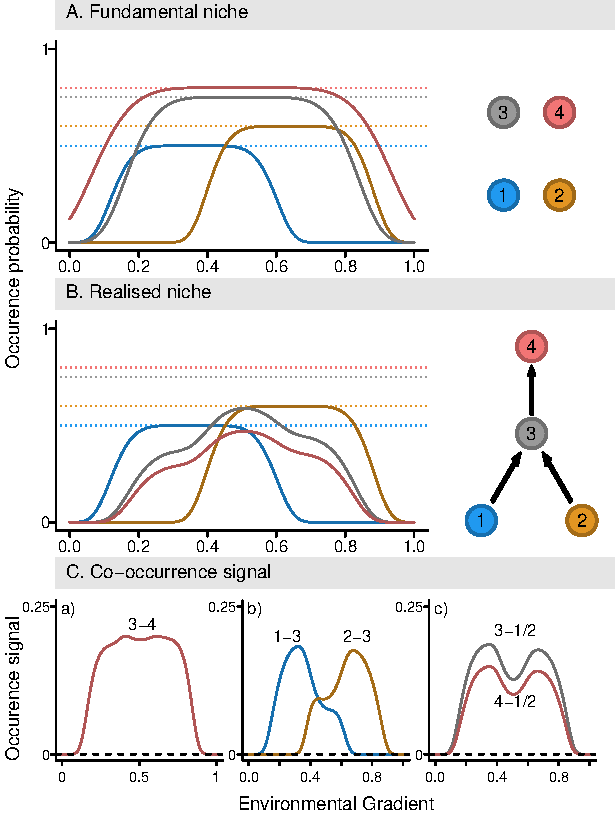
\includegraphics[width=0.87000\textwidth]{chapitre3/figConcept.pdf}
\caption{\textbf{Probabilistic description of fundamental and realized
niches} For a four species network, all the occurrence probabilities are
derived along an environmental gradient assuming that (A) interactions
are not limiting the distribution and (B) that predators 3 and 4 needs
at least of one of its preys, \emph{i.e.} species 1 or 2. Horizontal
dotted lines in (A) and (B) stand for the occurrence probabilities
reached at an environmental optimum. The co-occurrence signal is
calculated for the following pairs : a) predators 3 and 4; b) predator 3
and prey 1, predator 3 and prey 1; c) predator 3 and prey 1 or 2,
predator 4 and prey 1 or 2. If no difference are found, 0 is
expected.\label{fig:box1}}
\end{figure}

\newpage

\begin{figure}
\centering
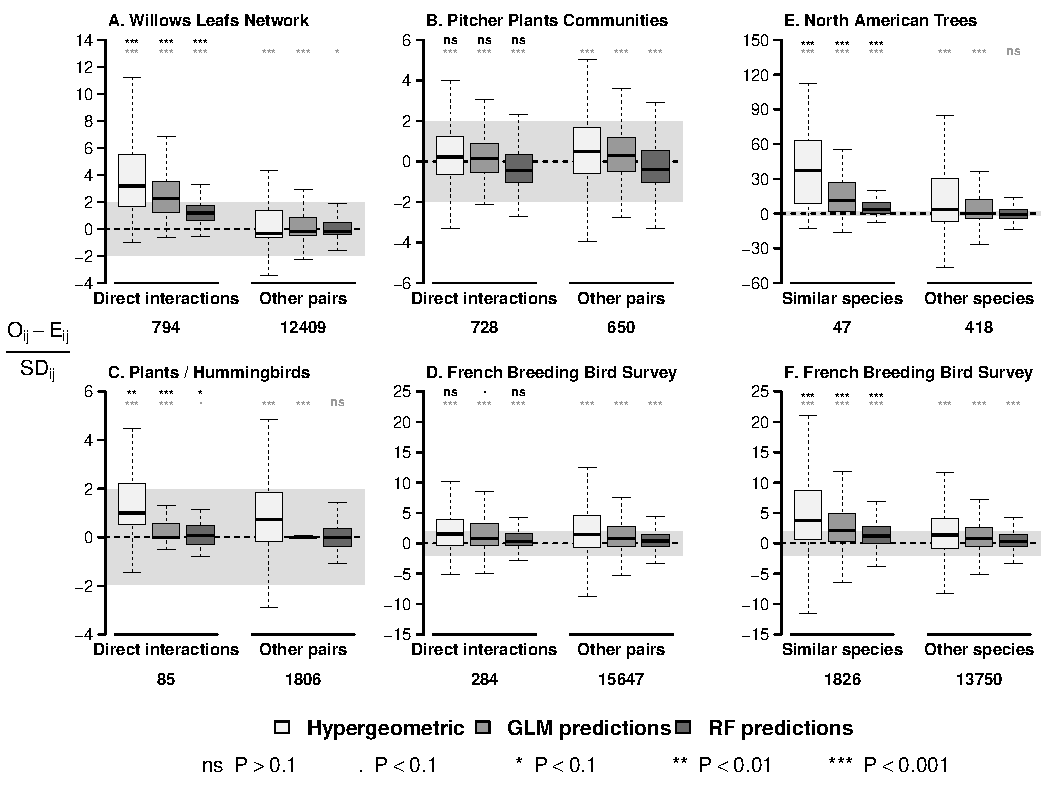
\includegraphics[width=0.95000\textwidth]{chapitre3/figIntVsNoint.pdf}
\caption{\textbf{Co-occurrence of interacting versus not-interacting
pairs of species} Figures under each groups of boxplots indicate the
number of pairs to which the Z-score distributions refer. The light grey
rectangle corresponds to the 95\% confidence interval for the standard
normal distribution which gives insight into the proportion of pairs of
species significantly different from 0. The comparison made in panels A
to D is based on direct interactions observed. For panels E and F,
similar species are defined as the species for which the trait-based
distance is less than or equal to the lower decile of this distance
distribution. Note that outliers are not displayed. P values were
computed using the Wilcoxon rank sum test, to compare interacting versus
not-interacting Z-score distribution calculated for the three different
methods (black symbols) and to show whether the distribution is
symmetric about 0 (light grey symbols).\label{fig:synth}}
\end{figure}

\newpage

\begin{figure}
\centering
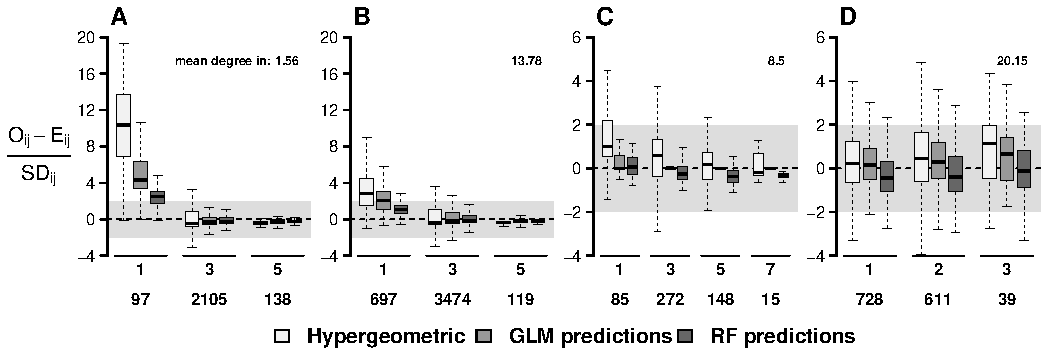
\includegraphics[width=0.95000\textwidth]{chapitre3/figOrder.pdf}
\caption{\textbf{Co-occurrence signal decays when the shortest path
between a pair of species decay} The Z-score distribution are plotted
against the shortest path for A willows-herbivores interactions, B
herbivores-parasitoids interactions, C birds-plants interactions and D
the pitcher plants network. First figures under each grouped boxplots
indicate the shortest path associated while the figures below provide
the number of pair to which the distribution refers. Note that we used
the same y-axis for panels A and B as they regard two different kind of
interaction of the same dataset.\label{fig:shtpth}}
\end{figure}

\newpage

\begin{figure}
\centering
\includegraphics[width=0.87000\textwidth]{chapitre3/figdegocc.pdf}
\caption{\textbf{Co-occurrence significance decreases as the cumulated
occupancy increases} For a given species, Z-scores are averaged over the
all set species it interacts with and plotted against the joint
distribution of the same set of species. We do so for the herbivores in
the willows leafs network (panels A to C), the parasitoids in the willow
leafs network (panels D to F), the hummingbirds in the Caribbean
hummingbirds datasets (panels G to I) and all species in the pitcher
plants network that consume other species (panels J to L). The x-axis is
expressed as a log proportion of the total number of sites. Black
symbols are mean Z-scores significantly different from 0 (see SI
\ref{chap3si}). In each panel, the dotted line represents the linear
regression \(y~ax+b\) for which the \(R^2\) is provided. The size of
circles reflects the degree of species for which the Z-score was
calculated, the relation size-degree for each row is given in the middle
panel. For the hummingbirds dataset (panels G to I), the triangle
represent the values obtained for the former distribution of a species
already analyzed (see SI \ref{chap3si}).\label{fig:degocc}}
\end{figure}

\newpage

\section{Supporting Information}\label{supporting-information}

\label{chap3si}

\subsection{Material and methods}\label{material-and-methods-1}

In this section, we present in more details, the datasets and the
methodology we used. All analyses have been performed using the R
environment software and Table \ref{tbl:rpkges} present the functions
and packages we used.

\subsubsection{Datasets}\label{datasets-1}

Sites for the five datasets are reported on five maps gathered in Fig.
\ref{fig:maps} The total number of species, the number of species
present in at least 1\% of the total number of sites and the number of
species for which traits information were available are reported in
Table \ref{tbl:numsp}.

\paragraph{Pitcher Plants Network}\label{pitcher-plants-network}

\emph{Sarracenia purpurea} is a carnivorous plant that occurs along the
east coast of North America from the panhandle of Florida to Canada and
across southern Canada to British Columbia \citep{Buckley2010}. \emph{S.
purpurea} has tube-shaped leaves that fill with rainwater and house a
food web consisting of bacteria, protozoa, rotifers, and dipteran larvae
among other taxa \citep{Addicott1974, Buckley2010}. This inquiline food
web decomposes prey items releasing nutrients to the plant
\citep{Mouquet2008, Baiser2011}. We used pitcher plant data from 39
sites across North America (Fig. 1B) collected by \citet{Buckley2010}.
This dataset contains abundance data and feeding interactions for 20
pitcher plant food webs at each site for a total of 769 food webs (11
pitchers were dropped due to missing data). In total, there are 90
species and morpho species. Interaction structure (\emph{i.e.}, who eats
whom) is from \citet{Baiser2012} which is based on previous studies
\citep[\emph{e.g.},][\citet{Butler2008}]{Addicott1974, Miller2002} and
direct observation of feeding interactions.

\paragraph{North American Trees}\label{north-american-trees}

We used a distance built upon nine functional traits whose values were
retrieved from \citep{Paquette2011}, see Supplementary Table
\ref{tbl:trees} available at
\url{http://onlinelibrary.wiley.com/doi/10.1111/j.1466-8238.2010.00592.x/suppinfo}.
Each of the nine selected variables were centered and scaled (R
functions used reported in Table \ref{tbl:rpkges}) then used as is to
derive Euclidean distances for all pairs of species. Then, we used
agglomeration clustering with the Ward's method (implemented in the
\emph{hclust()} function, see Table \ref{tbl:rpkges}) to obtain the
dendrogram presented in \ref{fig:dendro}.

\paragraph{French Breeding Birds Survey
datasets}\label{french-breeding-birds-survey-datasets}

We used 73 traits that are boolean variables reported in Table
\ref{tbl:trtfbbs} based on which we derive Euclidean distances between
all pairs of species.

\subsubsection{Building metawebs}\label{building-metawebs}

For four datasets, we built network based on all observed interactions
and derived associated quantities, \emph{i.e.} the connectance of the
metawebs, the degrees of species and the shortest-path, using the R
package \emph{igraph} (Table \ref{tbl:rpkges}).

\subsection{Co-occurrence measurement}\label{co-occurrence-measurement}

As mentioned in the main text, for three different scenarios, we derive
a standardized co-occurrence: for a given pair of species \(i\) and
\(j\), we examined \(\frac{O_{i,j}-E_{i,j}}{SD_{i,j}}\). Here, we
provide more information about the three methods wed used to analyze
co-occurrence.

\subsection{Hypergeometric
distribution}\label{hypergeometric-distribution}

This distribution has been mentioned in a different context
\citep[see][]{Gilpin1982} and has been fully exploited in
\citet{Veech2013} despite the author never referring to it as a
classical distribution. To clarify this, we start from the distribution
written in equation (1) in \citet{Veech2013}. We consider the
co-occurrence of two species on \(n\) sites. Species 1 is present in
\(n_1\) while species 2 is present in \(n_2\). The probability of having
\(j\) co\_occurrence, \(p_j\) is:

\[ p_j= \frac{\binom{n}{j} \binom{n-j}{n_2-j} \binom{n-n_2}{n_1-j}}{\binom{n}{n_2} \binom{n}{n_2}} \]

if \(\max{0, n_1+n_2-n} \leq j \leq \min{n_1, n_2}\) and 0 otherwise.
The expression above yields:

\[ p_j= \frac{n!}{(n-j)!j!} \frac{(n-j)!}{(n-j-n_2+j)!(n_2-j)!} \frac{(n-n_2)!}{(n-n_2-n_1+j)!(n_1-j)!} \frac{(n-n_1)!n_1!}{n!} \frac{1}{\binom{n}{n_2}} \]

by rearrangement:

\[ p_j= \frac{1}{j!} \frac{1}{(n_2-j)!} \frac{1}{(n-n_2-n_1+j)!(n_1-j)!} \frac{(n-n_1)!n_1!}{1} \frac{1}{\binom{n}{n_2}} \]

once sorted out, this yields:

\[ p_j= \frac{\binom{n_1}{j} \binom{n-n_1}{n_2-j}}{\binom{n}{n_2}} \]

Thus, the number of co-occurrence follows a hypergeometric distribution
of parameters \((n,n_1,n_2)\), which we used to calculate the expected
co-occurrence \(E_{i,j}\) under the hypothesis that all sites were
identical for all species.

\subsection{GLM and RF}\label{glm-and-rf}

For GLM and RF, \(E_{i,j}\) corresponds to probabilities of occurrence
computed based on climatic data. R functions are reported in Table
\ref{tbl:rpkges}.

\subsubsection{Climatic data}\label{climatic-data}

We used the global climate layers provided by the data WolrdClim,
version 1.4, available online at \url{http://www.worldclim.org}
\citep{Hijmans2005}. For each dataset, we performed a principal
component analysis and kept as many axes as needed to explain 90\% of
the total inertia. We used these axes for GLMs and RFs.

\subsubsection{Generalized Linear Model}\label{generalized-linear-model}

For all datasets, we performed a Generalized Linear Model
\citep{Elith2006} using all the axes provided by the PCA as polynomials
of degree 2. To constrain the number of parameters, we did not evaluate
the interactions among axis. We also performed model selection based on
the Akaike's information criterion (AIC) in a Stepwise Algorithm
\citep{burnham2013model}. R functions used to carry out the analyses are
indexed in Table \ref{tbl:rpkges}.

\subsubsection{Random Forests}\label{random-forests}

Random Forests \citep{Prasad2006} were performed using the same formula
as for GLMs. For all species, 10000 trees were computed and the
probability of a species being in a given site were calculated based on
the number of votes the sites were granted.

\subsubsection{Evaluating the models}\label{evaluating-the-models}

For all species, we assessed the performance of the Species Distribution
Models, \emph{i.e.} Generalized Linear Model and Random Forest, using
the Area Under the Receiver Operating Characteristic
\citep[AUROC,][]{Elith2006}. We present the results as a cumulative sum
of frequencies corresponding to the score for all species for each of
the four ecological systems we studied (see Fig. \ref{fig:ratauc}).

\subsection{Supporting Tables}\label{supporting-tables}

\subsubsection{R packages used}\label{r-packages-used}

\begin{longtable}[]{@{}lrrrr@{}}
\caption{R and packages used for the analyses. GLM: Generalized Linear
Model, PCA: Principal Component Analysis. AUROC: Area Under the Receiver
Operating Characteristic. \label{tbl:rpkges}}\tabularnewline
\toprule
Analysis & Function & Package name & Version & Citation\tabularnewline
\midrule
\endfirsthead
\toprule
Analysis & Function & Package name & Version & Citation\tabularnewline
\midrule
\endhead
Scaling and Centering & scale & base & 3.3.1 &
\citet{Rcoreteam2015}\tabularnewline
Euclidean distance & dist & stats & 3.3.1 &
\citet{Rcoreteam2015}\tabularnewline
Clustering & hclust & stats & 3.3.1 &
\citet{Rcoreteam2015}\tabularnewline
PCA & dudi.pca & ade4 & 1.7.4 & \citet{Dray2007}\tabularnewline
GLM & glm & stats & 3.3.1 & \citet{Rcoreteam2015}\tabularnewline
GLM Selection & step & stats & 3.3.1 &
\citet{Rcoreteam2015}\tabularnewline
Random Forests & randomForest & randomForest & 4.6.12 &
\citet{Liaw2002}\tabularnewline
Degree of species & degree & igraph & 1.0.1 &
\citet{Csardi2006}\tabularnewline
Shortest Paths & shortest.paths & igraph & 1.0.1 &
\citet{Csardi2006}\tabularnewline
AUROC & somers2 & Hmisc & 3.17.2 & \citet{HarrellJr2016}\tabularnewline
TSN retrieving & get\_tsn & taxize & 0.7.4 &
\citet{Chamberlain2013}\tabularnewline
Wilcoxon tests & wilcox.test & stats & 3.3.1 &
\citet{Rcoreteam2015}\tabularnewline
\bottomrule
\end{longtable}

\begin{longtable}[]{@{}lrrr@{}}
\caption{For each datasets we provide the total number of species
(column \emph{Total}), the number of species present in more that 1\% of
the total number of sites (column \emph{Selected}), and the number of
species for which traits information are available (column
\emph{Traits}). The symbol `-' means `not relevant'.
\label{tbl:numsp}}\tabularnewline
\toprule
Type & Total & Selected & Traits\tabularnewline
\midrule
\endfirsthead
\toprule
Type & Total & Selected & Traits\tabularnewline
\midrule
\endhead
Willow Leaf Network & 274 & 156 & - ~\tabularnewline
Pitcher Plants Network & 91 & 53 & -\tabularnewline
Caribbean Hummingbirds Network & 62 & 62 & -\tabularnewline
North American Trees & 31 & 31 & 31\tabularnewline
French Breeding Birds Survey & 340 & 179 & 321\tabularnewline
\bottomrule
\end{longtable}

\begin{longtable}[]{@{}lrrrrrrrrrr@{}}
\caption{Tree species and traits used. Abbreviations are as follows: TSN
- Taxonomic Serial Number defined by Integrated Taxonomic Information
System (ITIS), maxH - Average maximum height, GR - Growth rate, WD -
Wood Density,\\
TolS - Shade tolerance, TolD - Drought tolerance, AM - Arbuscular
mycorrhiza (Endomycorrhiza), EM - Ectomycorrhiza, LMA - Leaf mass per
area, Nmass - Nitrogen content per leaf mass unit \citep{Paquette2011}.
\label{tbl:trees}}\tabularnewline
\toprule
Species & TSN & maxH & GR & WD & TolS & TolD & AM & EM & LMA &
Nmass\tabularnewline
\midrule
\endfirsthead
\toprule
Species & TSN & maxH & GR & WD & TolS & TolD & AM & EM & LMA &
Nmass\tabularnewline
\midrule
\endhead
Abies balsamea & 18032 & 25 & 1 & 0.34 & 5.0 & 1.0 & 0 & 1 & 151.00 &
1.66\tabularnewline
Acer negundo & 28749 & 20 & 3 & 0.44 & 3.5 & 3.0 & 1 & 0 & 37.04 &
2.50\tabularnewline
Acer rubrum & 28728 & 25 & 3 & 0.49 & 3.4 & 1.8 & 1 & 0 & 71.09 &
1.91\tabularnewline
Acer saccharum & 28731 & 35 & 1 & 0.56 & 4.8 & 2.3 & 1 & 0 & 70.63 &
1.83\tabularnewline
Betula alleghaniensis & 19481 & 25 & 3 & 0.55 & 3.2 & 3.0 & 0 & 1 &
46.08 & 2.20\tabularnewline
Betula papyrifera & 19489 & 25 & 3 & 0.48 & 1.5 & 2.0 & 0 & 1 & 77.88 &
2.31\tabularnewline
Carpinus caroliniana & 19504 & 8 & 1 & 0.58 & 4.6 & 2.0 & 0 & 1 & 49.05
& 2.15\tabularnewline
Carya cordiformis & 19227 & 25 & 1 & 0.60 & 2.1 & 4.0 & 0 & 1 & 44.05 &
2.60\tabularnewline
Fagus grandifolia & 19462 & 25 & 1 & 0.56 & 4.8 & 1.5 & 0 & 1 & 61.22 &
2.04\tabularnewline
Fraxinus americana & 32931 & 30 & 2 & 0.55 & 2.5 & 2.4 & 1 & 0 & 76.75 &
2.12\tabularnewline
Fraxinus nigra & 32945 & 20 & 2 & 0.45 & 3.0 & 2.0 & 1 & 0 & 71.94 &
2.10\tabularnewline
Fraxinus pennsylvanica & 32929 & 25 & 3 & 0.53 & 3.1 & 3.9 & 1 & 0 &
87.72 & 1.80\tabularnewline
Larix laricina & 183412 & 25 & 3 & 0.48 & 1.0 & 2.0 & 0 & 1 & 120.00 &
1.36\tabularnewline
Ostrya virginiana & 19511 & 12 & 1 & 0.63 & 4.6 & 3.3 & 1 & 0 & 37.04 &
2.20\tabularnewline
Picea glauca & 183295 & 25 & 1 & 0.35 & 4.2 & 2.9 & 0 & 1 & 302.86 &
1.28\tabularnewline
Picea mariana & 183302 & 20 & 1 & 0.41 & 4.1 & 2.0 & 0 & 1 & 294.12 &
1.12\tabularnewline
Picea rubens & 18034 & 25 & 2 & 0.38 & 4.4 & 2.5 & 0 & 1 & 304.67 &
1.15\tabularnewline
Pinus banksiana & 183319 & 20 & 3 & 0.42 & 1.4 & 4.0 & 0 & 1 & 243.90 &
1.24\tabularnewline
Pinus resinosa & 183375 & 25 & 3 & 0.39 & 1.9 & 3.0 & 0 & 1 & 294.12 &
1.17\tabularnewline
Pinus strobus & 183385 & 30 & 3 & 0.36 & 3.2 & 2.3 & 0 & 1 & 121.92 &
1.42\tabularnewline
Populus balsamifera & 22453 & 25 & 3 & 0.37 & 1.3 & 1.8 & 1 & 1 & 83.46
& 1.95\tabularnewline
Populus grandidentata & 22463 & 20 & 3 & 0.39 & 1.2 & 2.5 & 1 & 1 &
70.45 & 2.50\tabularnewline
Populus tremuloides & 195773 & 25 & 3 & 0.37 & 1.2 & 1.8 & 1 & 1 & 82.02
& 2.16\tabularnewline
Prunus pensylvanica & 24799 & 12 & 3 & 0.36 & 1.0 & 2.0 & 1 & 1 & 50.00
& 2.40\tabularnewline
Quercus alba & 19290 & 35 & 1 & 0.60 & 2.9 & 3.6 & 0 & 1 & 81.21 &
2.39\tabularnewline
Quercus macrocarpa & 19287 & 15 & 1 & 0.58 & 2.7 & 3.9 & 0 & 1 & 92.74 &
2.27\tabularnewline
Quercus rubra & 19408 & 25 & 2 & 0.56 & 2.8 & 2.9 & 0 & 1 & 84.20 &
2.06\tabularnewline
Thuja occidentalis & 505490 & 15 & 1 & 0.30 & 3.5 & 2.7 & 1 & 0 & 223.00
& 1.02\tabularnewline
Tsuga canadensis & 183397 & 30 & 1 & 0.40 & 4.8 & 1.0 & 0 & 1 & 122.55 &
0.99\tabularnewline
Ulmus americana & 19049 & 35 & 3 & 0.46 & 3.1 & 2.9 & 1 & 0 & 79.47 &
2.07\tabularnewline
Ulmus rubra & 19050 & 25 & 3 & 0.48 & 3.3 & 3.0 & 1 & 0 & 59.88 &
2.50\tabularnewline
\bottomrule
\end{longtable}

\begin{longtable}[]{@{}lr@{}}
\caption{List of the Boolean traits used to compute Euclidean distances
between all pairs of species in the French Breeding Birds Survey.
\label{tbl:trtfbbs}}\tabularnewline
\toprule
Category & Trait name\tabularnewline
\midrule
\endfirsthead
\toprule
Category & Trait name\tabularnewline
\midrule
\endhead
Activity & Nocturnal\tabularnewline
Activity & Crepuscular\tabularnewline
Activity & Diurnal\tabularnewline
Diet & Seeds, nuts or grain\tabularnewline
Diet & Fruits / frugivory\tabularnewline
Diet & Vegetative\tabularnewline
Diet & invert\tabularnewline
Diet & fish\tabularnewline
Diet & Very small mammals\tabularnewline
Diet & Large mammals\tabularnewline
Diet & Herptile\tabularnewline
Diet & Small birds\tabularnewline
Diet & Long birds\tabularnewline
Diet & Vertebrate\tabularnewline
Diet & Bones\tabularnewline
Diet & Carrion\tabularnewline
Feeding behavior & Pursuit (air and/or aquatic)\tabularnewline
Feeding behavior & Sally\tabularnewline
Feeding behavior & Foliage gleaning\tabularnewline
Feeding behavior & Pouncing\tabularnewline
Feeding behavior & Grazing\tabularnewline
Feeding behavior & Picking, pecking or stabbing\tabularnewline
Feeding behavior & Digging\tabularnewline
Feeding behavior & Overturning\tabularnewline
Feeding behavior & Probing\tabularnewline
Feeding behavior & Filtering\tabularnewline
Feeding habitat & Water-surface\tabularnewline
Feeding habitat & Underwater\tabularnewline
Feeding habitat & Water\tabularnewline
Feeding habitat & Mud\tabularnewline
Feeding habitat & Ground\tabularnewline
Feeding habitat & Canopy\tabularnewline
Feeding habitat & Shrub (low and high)\tabularnewline
Feeding habitat & Vegetation\tabularnewline
Feeding habitat & Air\tabularnewline
Foraging habitat & Wet grassland, meadows, fens, sedges or
tundra\tabularnewline
Foraging habitat & Dry grassland\tabularnewline
Foraging habitat & Rocky slope\tabularnewline
Foraging habitat & Fast river/stream\tabularnewline
Foraging habitat & Slow river/stream\tabularnewline
Foraging habitat & Shore (marine)\tabularnewline
Foraging habitat & Salt marsh\tabularnewline
Foraging habitat & Mud or silt\tabularnewline
Foraging habitat & Sandy gravel/beach\tabularnewline
Foraging habitat & Reed marshes\tabularnewline
Foraging habitat & Conifer\tabularnewline
Foraging habitat & Mixed forest\tabularnewline
Foraging habitat & Deciduous\tabularnewline
Foraging habitat & Mediterranean oak or other\tabularnewline
Foraging habitat & Open/low forest\tabularnewline
Foraging habitat & Forest or habitat edge\tabularnewline
Foraging habitat & Shrub/bush\tabularnewline
Foraging habitat & Urban\tabularnewline
Foraging habitat & Garden\tabularnewline
Foraging habitat & High air\tabularnewline
Nesting habitat & Wet grassland, meadows, fens, sedges or
tundra\tabularnewline
Nesting habitat & Dry grassland\tabularnewline
Nesting habitat & Banks/sand/mud\tabularnewline
Nesting habitat & Rock surface/outcrops\tabularnewline
Nesting habitat & Near water/shore/island\tabularnewline
Nesting habitat & Sand gravel/beach\tabularnewline
Nesting habitat & Reed marshes\tabularnewline
Nesting habitat & Conifer\tabularnewline
Nesting habitat & Mixed forest\tabularnewline
Nesting habitat & Deciduous\tabularnewline
Nesting habitat & Mediterranean oak and other\tabularnewline
Nesting habitat & Open/low forest\tabularnewline
Nesting habitat & Shrub/bush\tabularnewline
Nesting habitat & Urban\tabularnewline
Nesting habitat & Garden\tabularnewline
Nesting location & Elevated\tabularnewline
Nesting location & Tree hole\tabularnewline
Nesting location & Ground\tabularnewline
\bottomrule
\end{longtable}

\newpage

\section{Supporting Figures}\label{supporting-figures}

\begin{figure}
\centering
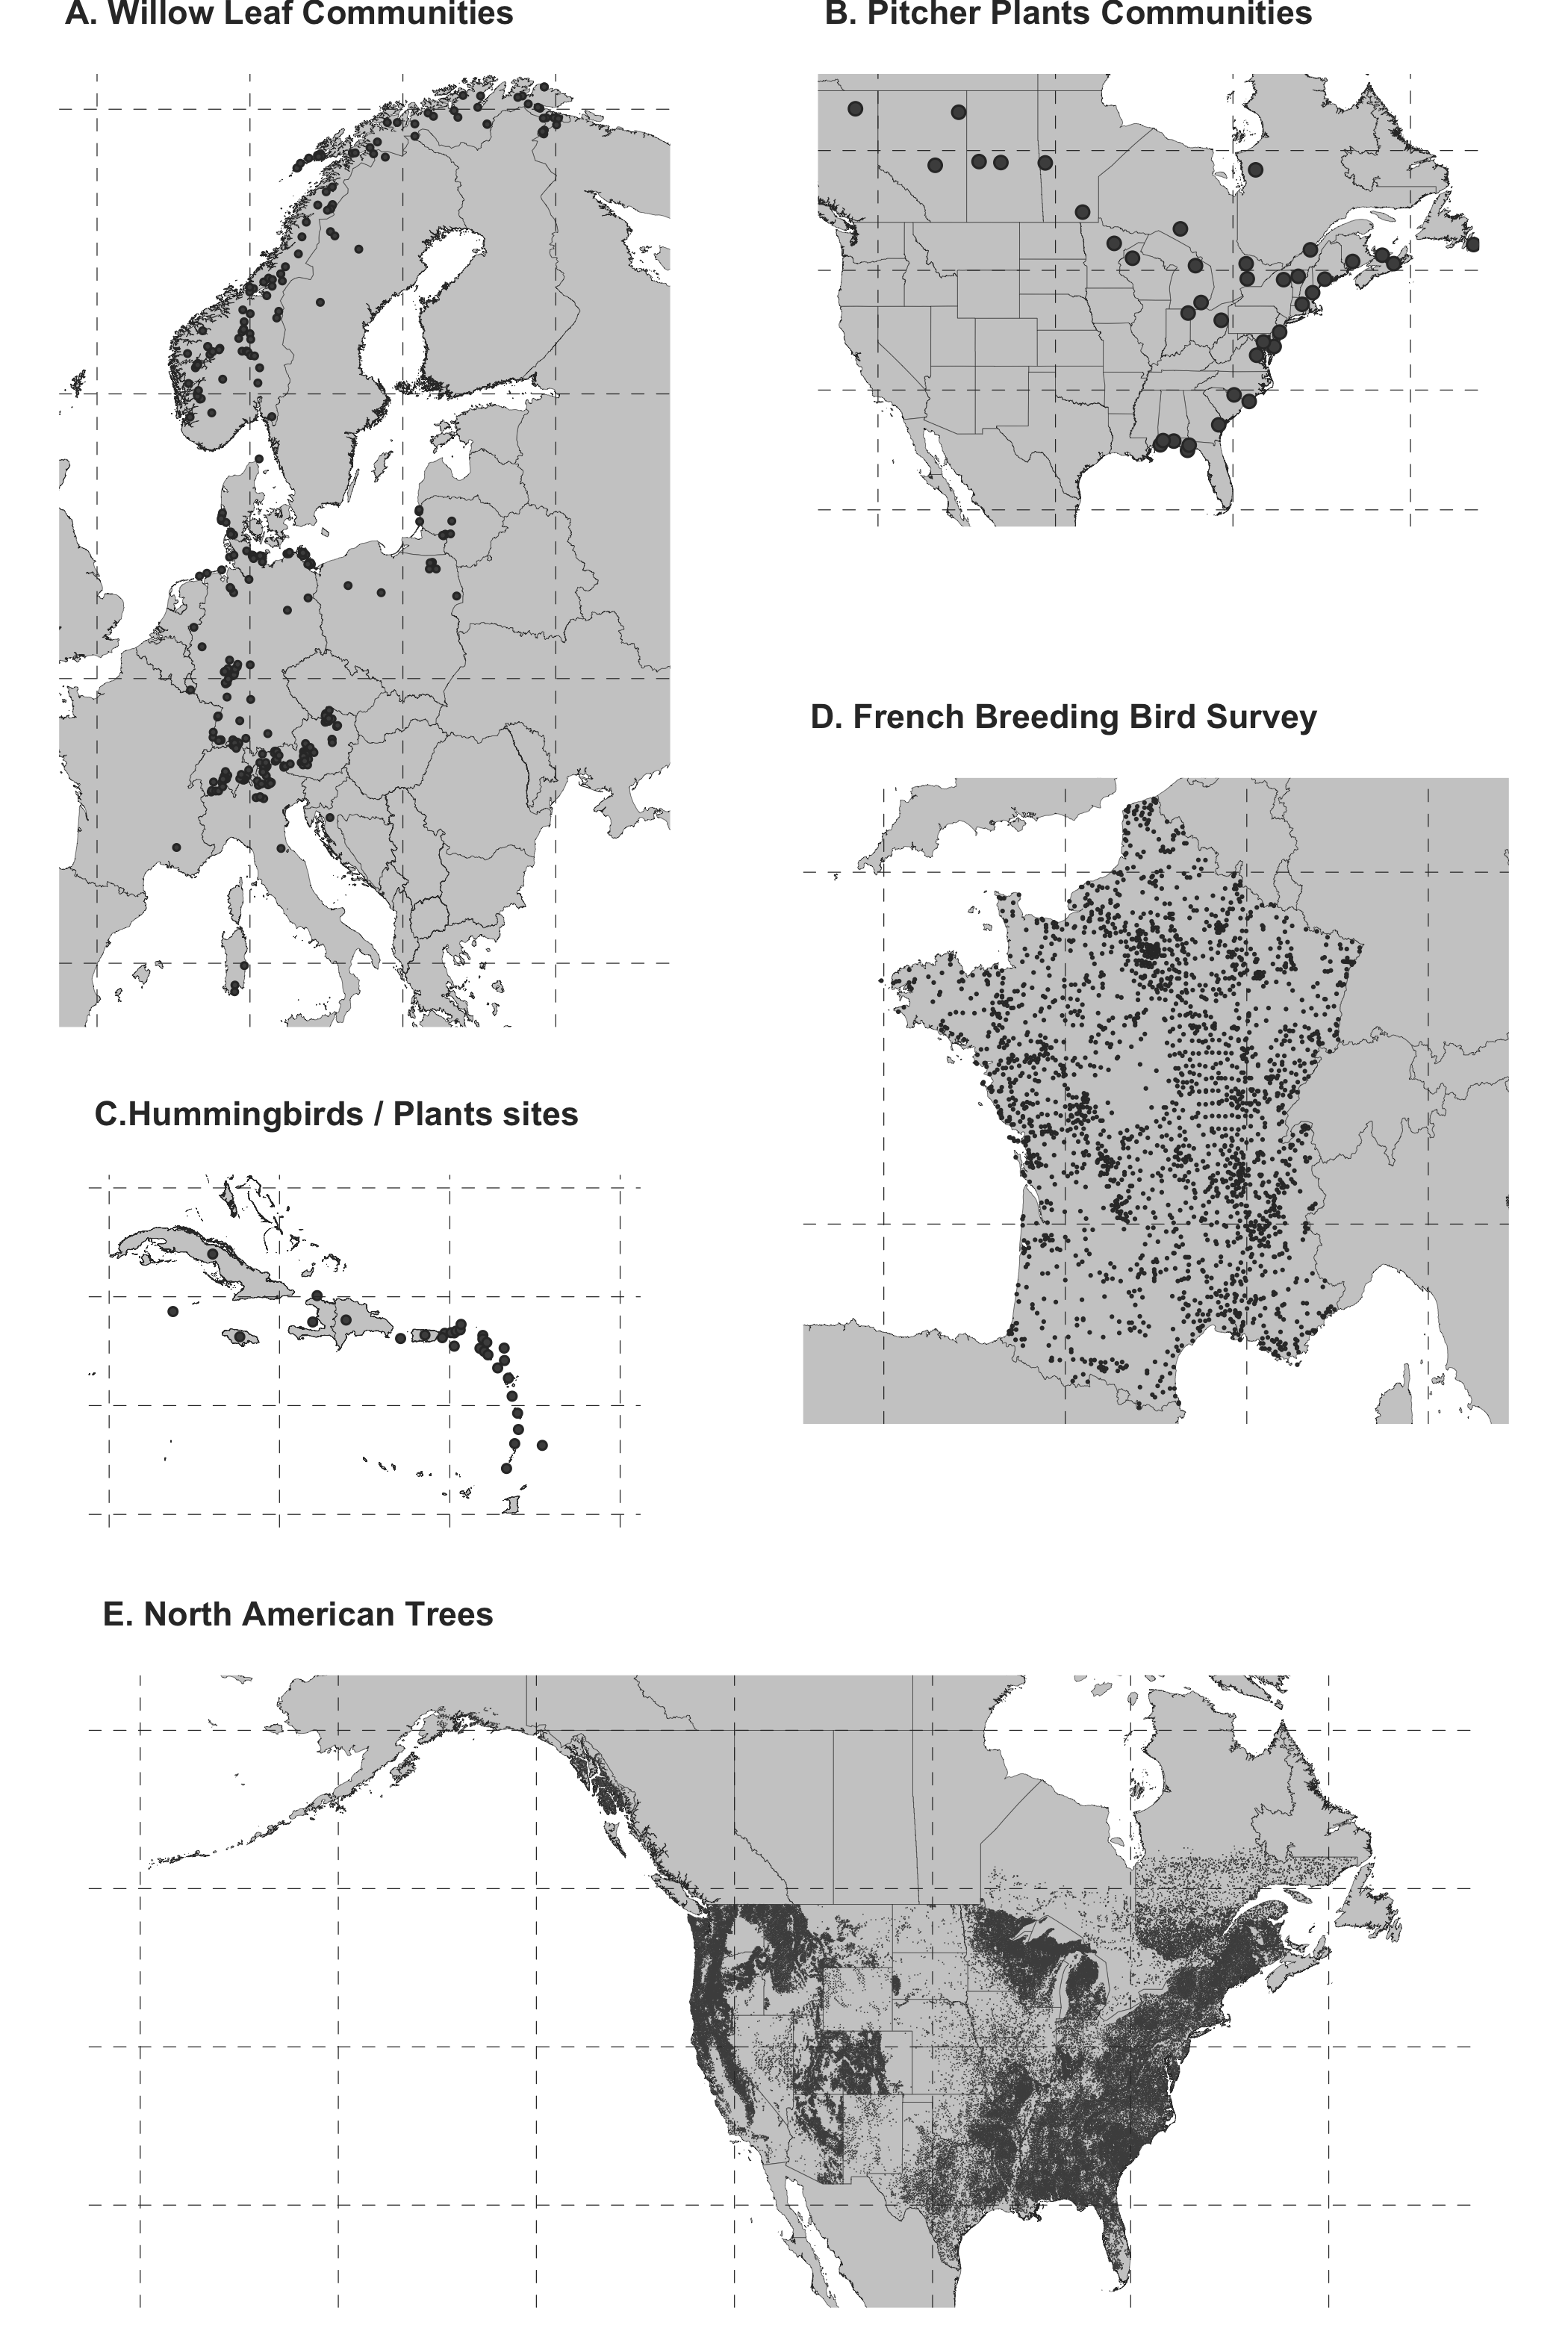
\includegraphics[width=0.90000\textwidth]{chapitre3/figS1.png}
\caption{\textbf{Sites of the study}\label{fig:maps}}
\end{figure}

\newpage

\begin{figure}
\centering
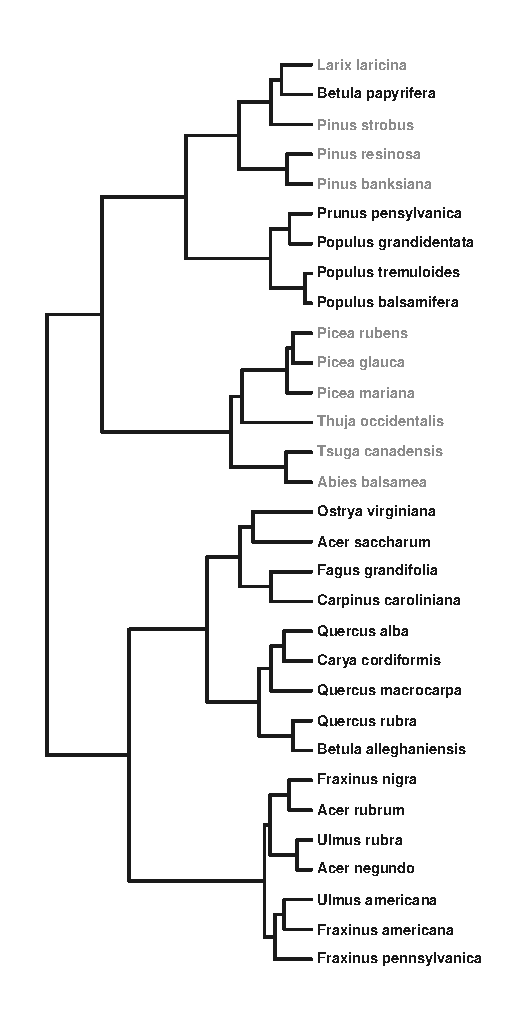
\includegraphics{chapitre3/figS2.pdf}
\caption{\textbf{Dendrogram representing the trait-based distances
between the 31 species studied in the North American tree datasets.}
Names of angiosperm species are written in dark grey while names of
Gymnosperm species are in a lighter grey.\label{fig:dendro}}
\end{figure}

\newpage

\begin{figure}
\centering
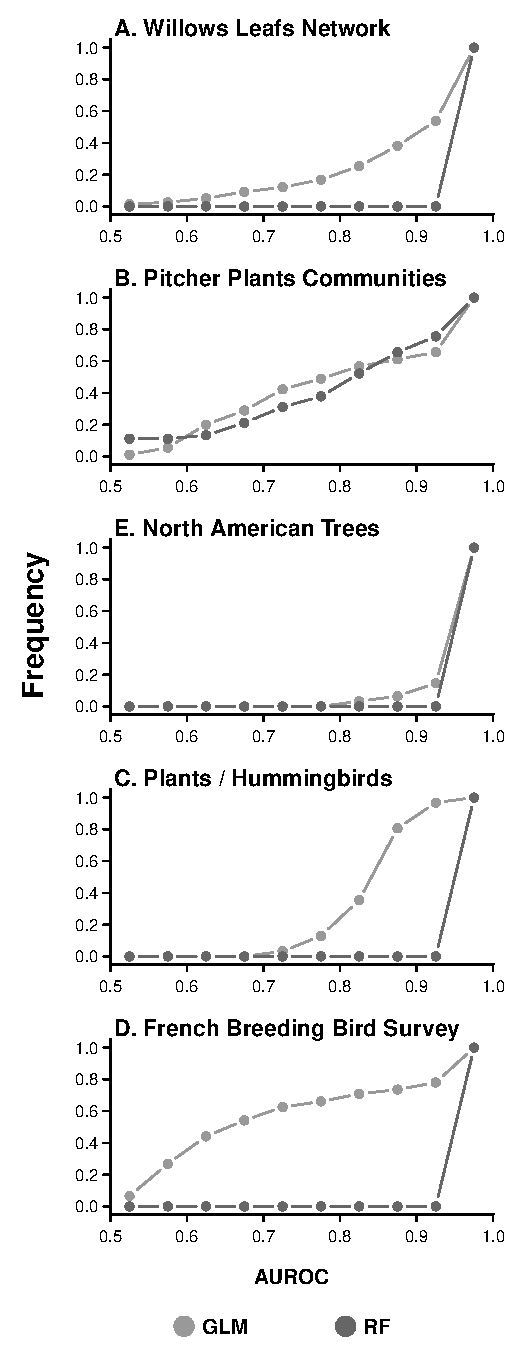
\includegraphics[width=0.50000\textwidth]{chapitre3/figS3.pdf}
\caption{\textbf{Evaluation of the SDMs} For each dataset, the
distributions of AUC for GLMs (light grey symbols) and RFs (dark grey
symbols) for all species are presented.\label{fig:auc}}
\end{figure}

\newpage

\begin{figure}
\centering
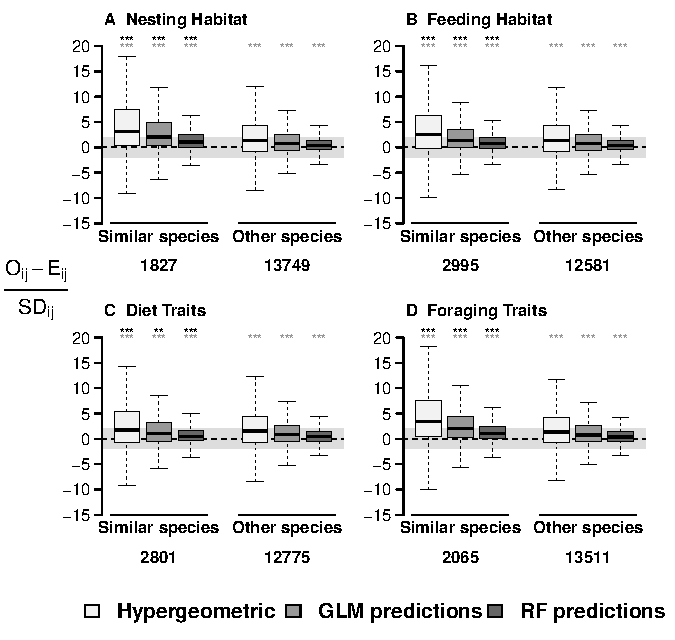
\includegraphics[width=0.95000\textwidth]{chapitre3/figS4.pdf}
\caption{\textbf{Co-occurrence and the nature of the trait-based
distance in the FBBS dataset} The different panels correspond to four
different set of trait upon which different distances are built. Similar
species are defined as the species for which the trait-based distance is
less than or equal to the lower decile of this distance distribution.
Note that outliers are not displayed. The light grey rectangle
corresponds to the 95\% confidence interval for the standard normal
distribution which gives insight into the proportion of pairs of species
significantly different from 0. P values were computed using the
Wilcoxon rank sum test, to compare interacting versus not-interacting
Z-score distribution calculated for the three different methods (black
symbols). They were also computed to show whether whether Z-score were
greater for hypergeometric versus GLM and GLM versus RF (grey
symbols).\label{fig:dist}}
\end{figure}

\newpage

\begin{figure}
\centering
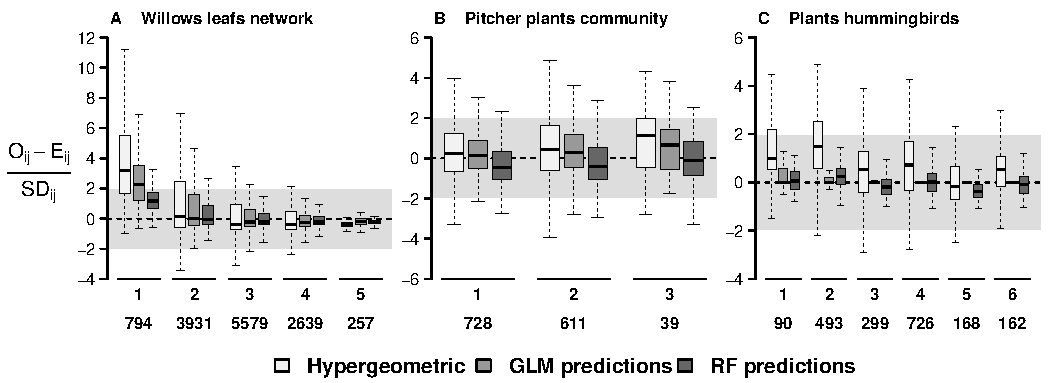
\includegraphics[width=0.95000\textwidth]{chapitre3/figS5.pdf}
\caption{\textbf{Co-occurrence signal decays when the shortest path
between a pair of species decay} Distribution of Z-scores for all
interactions are grouped by shortest-path indicated by the first numbers
below boxplots. The other figures below stand for the number of pairs of
species included within the distributions.\label{fig:sht_pth2}}
\end{figure}

\newpage

\begin{figure}
\centering
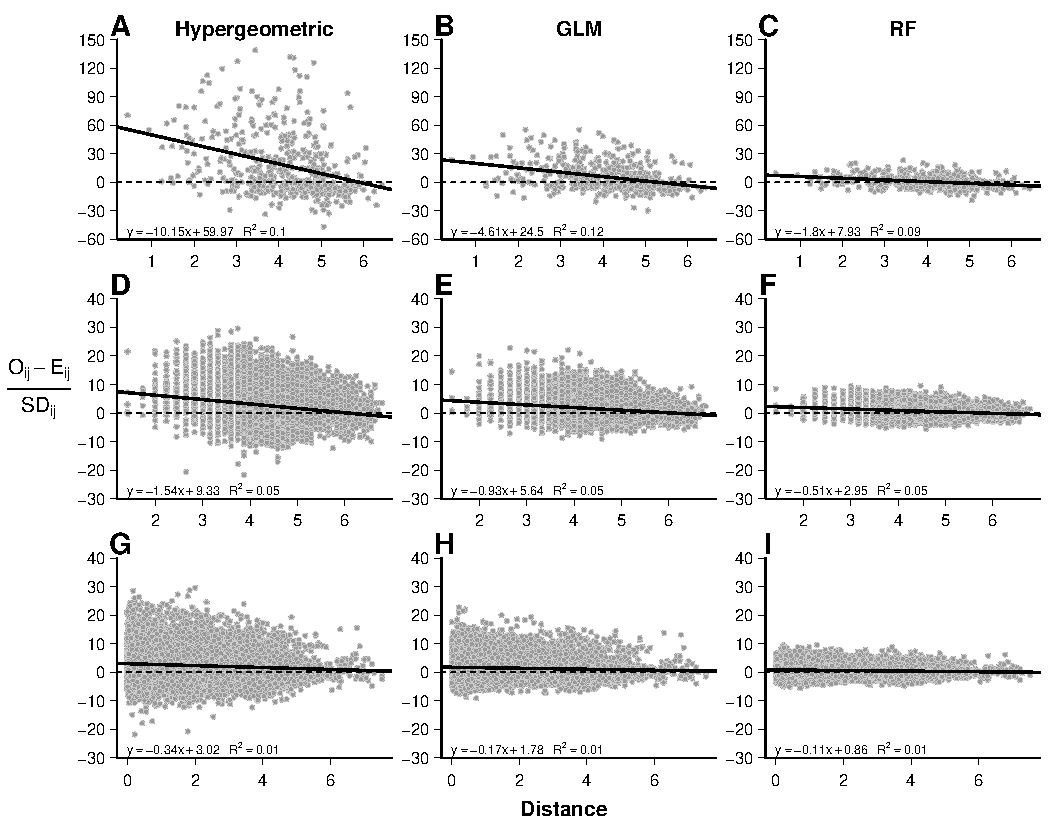
\includegraphics[width=0.95000\textwidth]{chapitre3/figS6.pdf}
\caption{\textbf{Changes in co-occurrence signal with increased distance
between two species} Points represent the result for all pairs of
interaction for two datasets: the North American Tree dataset (A=C) and
the FBBS (D-I). For the latter, we used the trait-based distance
computed with all available traits (D-F) and the body-size ratios (the
lighter species over the heavier, panels G-I). In each panel, the
equation on the bottom-left corner indicated the results of the linear
regression depicted by the dotted line.\label{fig:distrev}}
\end{figure}

\newpage

\begin{figure}
\centering
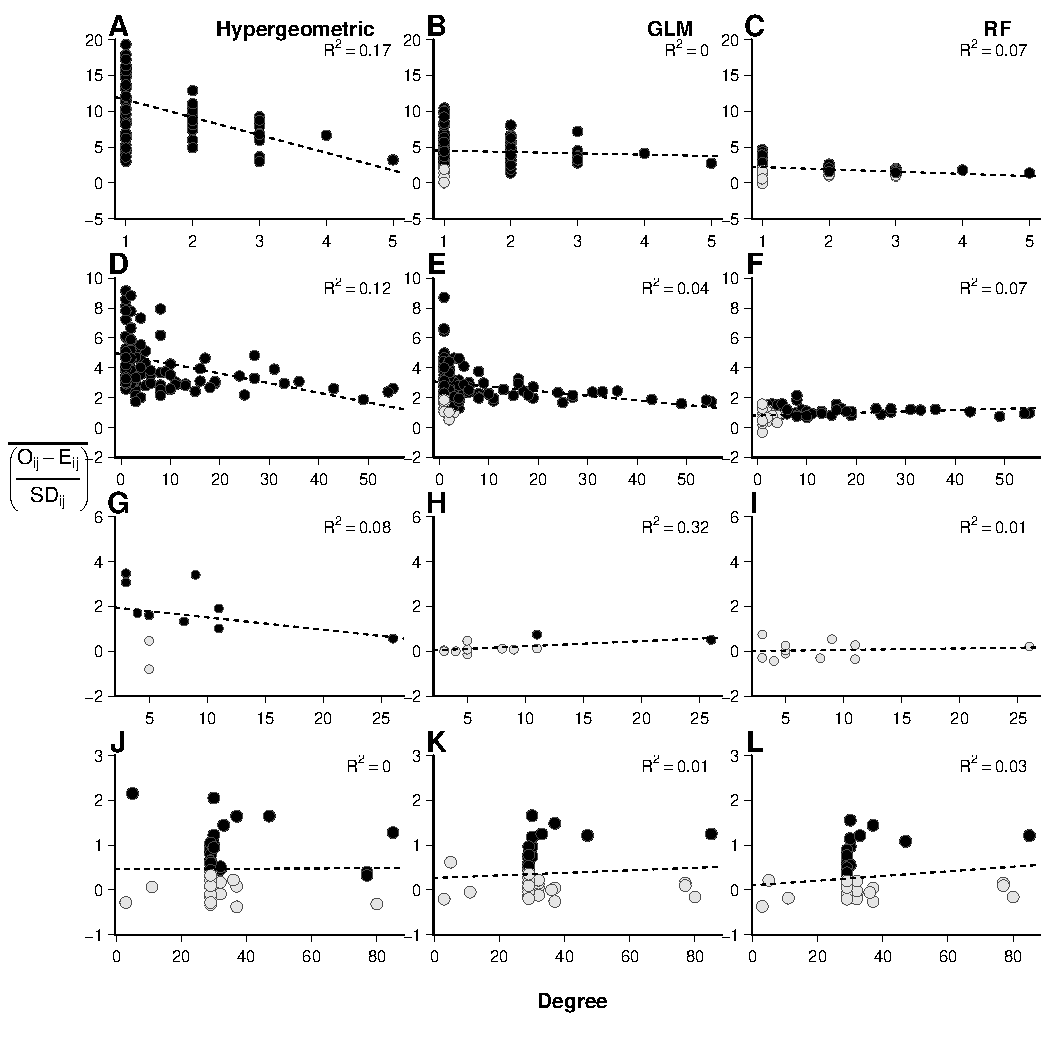
\includegraphics[width=0.95000\textwidth]{chapitre3/figS7.pdf}
\caption{\textbf{The degree of species partially explains the decrease
of the co-occurrence strength} For the herbivores (A-C) and the
parasitoids in the willow leafs network datasets (D-F), the hummingbirds
in the Caribbean hummingbirds datasets (G-I) and all species in the
pitcher plants network that consume other species (J-L) the mean Z-score
is plotted against the degree of the species. Black symbols are mean
Z-scores significantly different from 0 (see SI Text). In each panel,
the dotted line represents the linear regression \(y~ax+b\) for which
the \(R^2\) is provided.\label{fig:degree}}
\end{figure}

\newpage

\begin{figure}
\centering
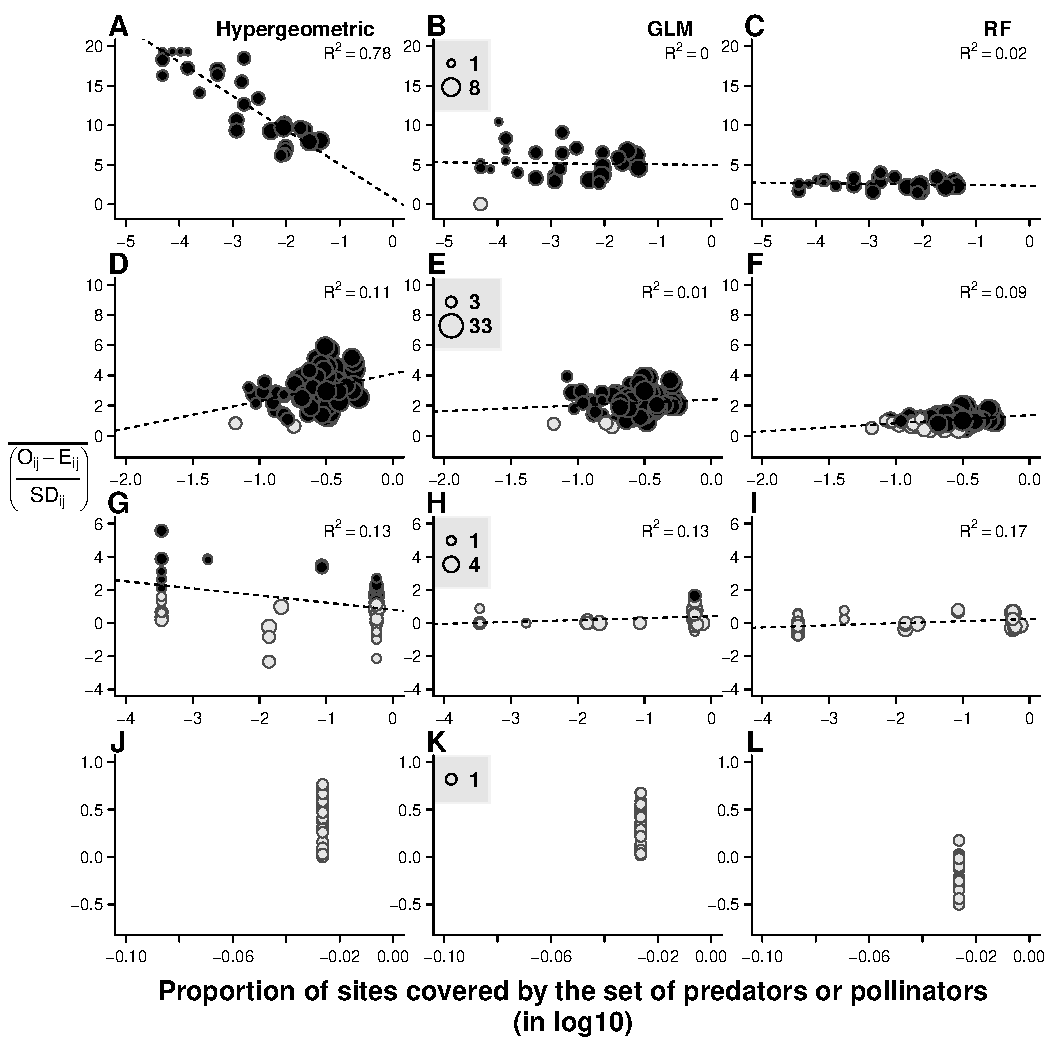
\includegraphics[width=0.95000\textwidth]{chapitre3/figS8.pdf}
\caption{\textbf{Reversed figure 4} This figure corresponds to figure 4
in the main text, but the Z-score were calculated for preys (host
plants) rather than for predators (pollinators). Mean Z-score are
computed for willows (A-C) and herbivores (based on the
herbivores-parasitoids only, D-F) of the willows leafs network, the
hosts plants in the Caribbean hummingbirds datasets (G-I) and species
that feed on the detritus in the pitcher plants network (panels J-L).
The x-axis is expressed as a log proportion of the total number of sites
included in the considered dataset. Black symbols are mean Z-scores
significantly different from 0 (see SI Text). In each panel, the dotted
line represents the linear regression \(y~ax+b\) for which the \(R^2\)
is provided. The size of circles reflects the degree of species for
which the Z-score was calculated, the relation size-degree for each row
is given in the middle panel.\label{fig:degocc2}}
\end{figure}

\newpage

\begin{figure}
\centering
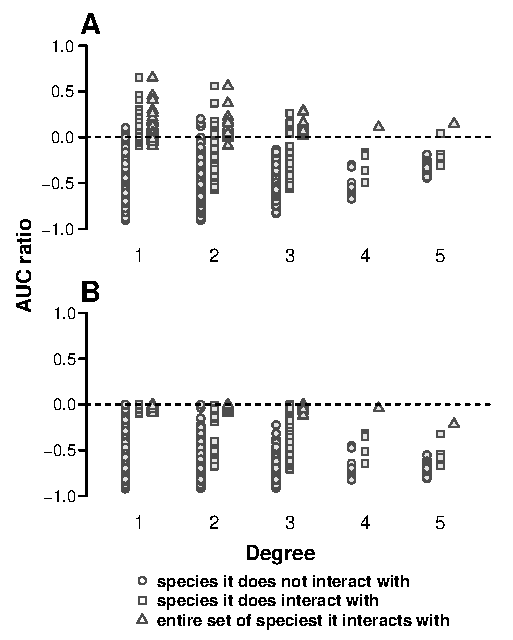
\includegraphics[width=0.95000\textwidth]{chapitre3/figS9.pdf}
\caption{\textbf{Predicting herbivore distribution based on the
distribution of willows} For the herbivores in the willow leafs network
dataset, we compared the AUC obtained when using willow it does not
interact with (circles) a willow in interacts with (squares) and the set
of willow it interacts with (triangles) to AUC obtained for GLM (A) and
RF (B). Positive values indicated that species based model outperformed
the SDM model.\label{fig:ratauc}}
\end{figure}
